\chapter{Urlaubsverwaltung}
\label{urlaubsverwaltung}
\section{Allgemeines}

Die Urlaubsverwaltung ist unter "`Mein CIS"' Urlaubstool zu finden.
Das Urlaubstool dient als Erweiterung der Zeitsperren (siehe Kapitel \ref{zeitsperren_zeitwuensche}), um diese leichter und �bersichtlicher eintragen zu k�nnen.

\begin{itemize}
	\item Der Abrechnungszeitraum f�r die Urlaubserfassung ist von 01.09. eines Jahres bis zum 31.08. des Folgejahres.
	\item Der Urlaubsanspruch eines/einer MitarbeiterIn wird von der Gesch�ftsstelle administriert und gewartet.
	\item Der/die MitarbeiterIn tr�gt im Laufe des Jahres im Urlaubstool seine/ihre gew�nschten Urlaubstage ein.
	\item Der/die - in der Datenbank zugeteilte - InstitutsleiterIn bzw. Vorgesetzte erh�lt daraufhin eine E-Mail mit einem Freigabeansuchen. Nach der Freigabe kann der eingetragene Urlaub nicht mehr durch den/die MitarbeiterIn bearbeitet werden.
	\item Mit Stichtag 31.08. wird der aktuelle Urlaubsanspruch ermittelt. Dazu tr�gt der/die InstitutsleiterIn/Vorgesetzte die aktuellen Resturlaubstage in das System ein. Diese werden mit dem derzeitigen Urlaubsanspruch addiert und ergeben, abz�glich des aktuell gebuchten Urlaubs, den Urlaubsanspruch ab 01.09.
	\item Der/die MitarbeiterIn kann diese Berechnung auf der CIS-Seite einsehen.
	\item Bei fehlender oder falscher Institutszuordnung wenden Sie sich bitte an die Personalabteilung. 
\end{itemize}

\begin{figure}
	\centering
	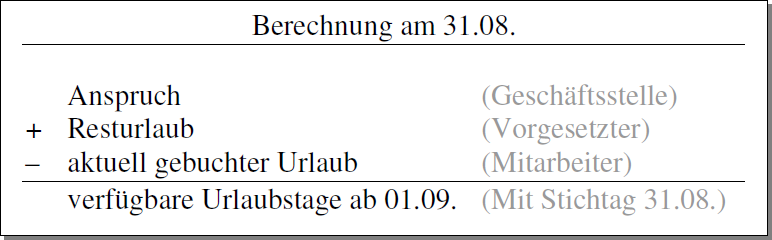
\includegraphics[width=0.70\textwidth]{CIS_Urlaubstool_Berechnung.png}
	\caption{Berechnung der Urlaubstage}
\end{figure}

\section{Verwendung des Tools}

Das Urlaubstool wird �ber die CIS-Seite aufgerufen und dient als Erweiterung der bisherigen Eingabemaske der Zeitsperren. Sie k�nnen weiterhin Zeitsperren wie gewohnt eintragen und bearbeiten.
Wir empfehlen, Mozilla Firefox oder SeaMonkey als Browser zu verwenden.

\subsection{Buchen eines Urlaubs}

Der �bersicht oben links (siehe Abbildung \ref{CIS_urlaubstool_eintragungen}) k�nnen Sie Ihren aktuellen Urlaubsanspruch und dessen Berechnung entnehmen. Mit dem Hilfe-Button erhalten Sie eine detaillierte
Erl�uterung der Berechnung.

\begin{figure}
	\centering
	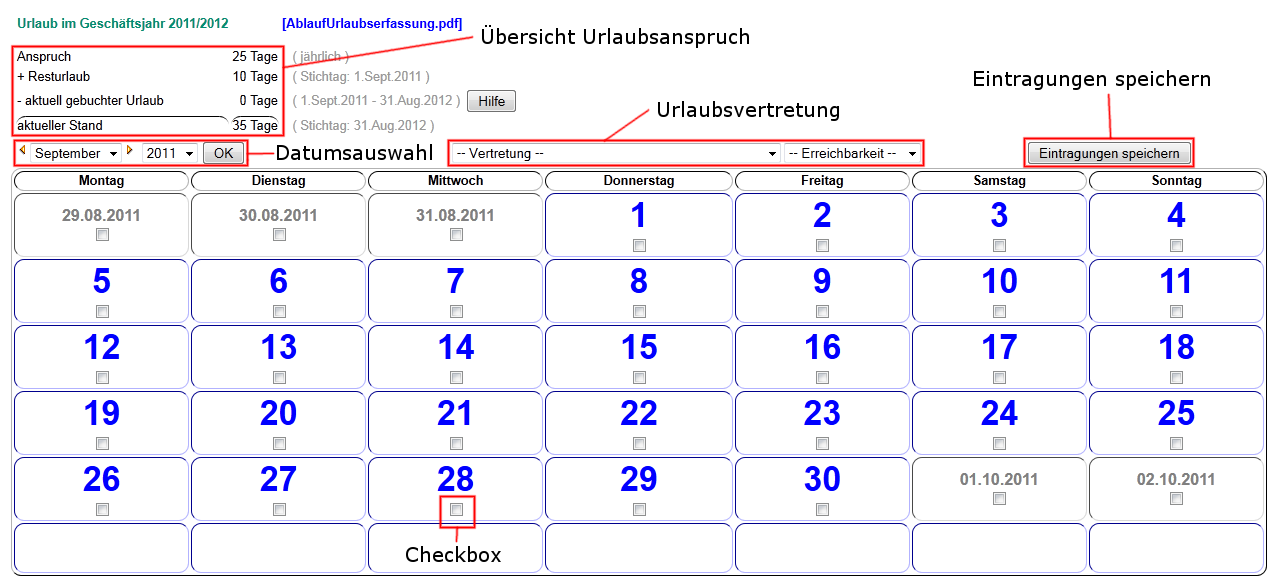
\includegraphics[width=1\textwidth]{CIS_Urlaubstool_Eintragungen.png}
	\caption{Eintragungen speichern}
	\label{CIS_urlaubstool_eintragungen}
\end{figure}

W�hlen Sie nun das gew�nschte Monat und Jahr aus, in dem Sie den Urlaub eintragen m�chten. Dies k�nnen Sie direkt mittels Auswahl aus den Drop-Down-Feldern und \textbf{dr�cken des OK-Buttons} oder durch Bl�ttern mit den gelben Pfeiltasten.

Sie sehen unter jedem Wochentag Checkboxen, die Sie durch einen einfachen Klick mit der Maustaste an- und abw�hlen k�nnen. Markieren Sie nun auf diese Weise die Tage, an denen Sie Ihren Urlaub konsumieren m�chten.

\achtung{Es werden zur Zeit noch keine Feiertage angezeigt. Kontrollieren Sie bitte selbstst�ndig, ob ein Feiertag innerhalb Ihres Urlaubs liegt.}

W�hlen Sie nun aus den Drop-Down-Feldern Ihre Urlaubsvertretung aus und wie Sie f�r die Zeit Ihres Urlaubs erreichbar sind. 
Wenn Sie nichts angeben, wird automatisch "`Nicht erreichbar!"' gespeichert. Dr�cken Sie nun \textbf{Eintragungen speichern}. 

Der gebuchte Urlaub erscheint nun in Hellgr�n im Kalender. Gleichzeitig wird eine
E-Mail mit dem Freigabeansuchen an Ihren Vorgesetzten versendet, was Ihnen auch unterhalb des Kalenders durch einen roten Infotext best�tigt wird.

\info{Sollte kein/e Vorgesetzte/r in der Datenbank zugeordnet sein, so steht dies ebenfalls im Infotext. Kontaktieren Sie in diesem Fall bitte die Personalabteilung.}

Wenn Sie mit dem Cursor auf einem gebuchten Urlaub zu stehen kommen (auf der Zahl) erscheint im Quickinfo die gespeicherte Vertretung und Erreichbarkeit.

\begin{figure}
	\centering
	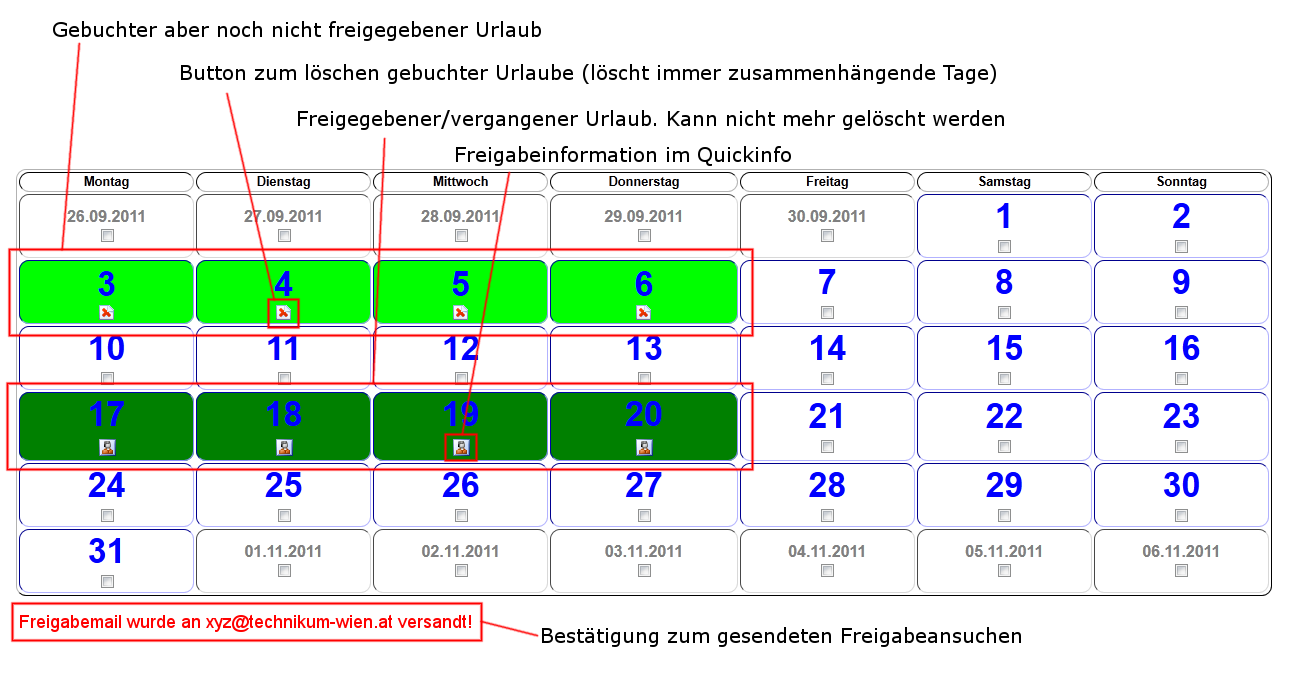
\includegraphics[width=1\textwidth]{CIS_Urlaubstool_Buchungen.png}
	\caption{Eingetragener Urlaub}
	\label{CIS_urlaubstool_buchungen}
\end{figure}

\section{L�schen eines gebuchten Urlaubs}

Einen gebuchten und noch NICHT freigegebenen Urlaub, k�nnen Sie durch klicken auf das x unterhalb eines jeden Eintrags l�schen.
Zusammenh�ngende (aufeinander folgende) Tage werden als solche gespeichert und auch entsprechend wieder gel�scht. Ein Klick auf den L�schen-Button in Abbildung \ref{CIS_urlaubstool_buchungen},
w�rde also den Urlaub vom 03.-06.August l�schen.

\textit{Bitte buchen Sie Ihren Urlaub �berlegt, um Ihrem/Ihrer Vorgesetzten eine Flut an Mails zu ersparen und unn�tige Verwirrungen zu vermeiden.}

\section{Freigegebener Urlaub}

Nachdem Ihr/e Vorgesetzte/r Ihren gew�nschten Urlaub freigegeben hat, erscheint er im Urlaubstool dunkelgr�n und kann nicht mehr von Ihnen gel�scht werden.
Das L�schen-Symbol ist nun durch ein Informations-Icon ersetzt worden und im Quickinfo des Symbols erhalten Sie die Information, wann und von wem der Urlaub freigegeben worden ist.

\achtung{Wenn Sie nachtr�glich einen Urlaub in der Vergangenheit buchen (vor dem heutigen Datum), wird dieser automatisch als freigegeben markiert und kann nicht mehr gel�scht werden.}

